\section*{Supplementary Materials (Tables S1--S6 and Figure S1)}
\renewcommand{\thetable}{S\arabic{table}}
\setcounter{table}{0}
\renewcommand{\thefigure}{S\arabic{figure}}
\setcounter{figure}{0}
% Unique PDF anchors after restarting supplementary figure/table numbering.
\renewcommand{\theHfigure}{supp.\arabic{figure}}
\renewcommand{\theHtable}{supp.\arabic{table}}

\begin{figure}[!htbp]
\centering
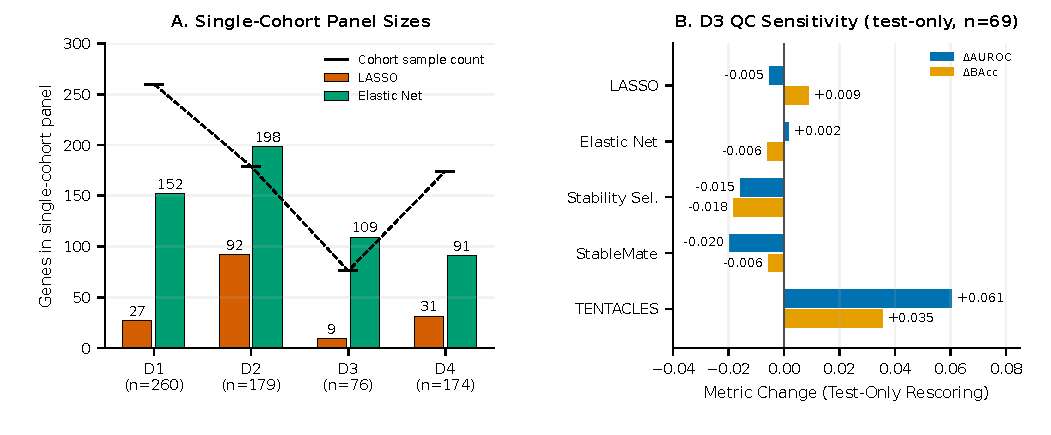
\includegraphics[width=\textwidth]{panel_sizes_and_d3_qc_sensitivity.pdf}
\caption{(A) Single-cohort LASSO and Elastic Net panel sizes relative to cohort sample counts, illustrating model sparsity. (B) Held-out D3 QC sensitivity: test-only rescoring excluding the seven source-flagged \texttt{qc=EXCLUDE} samples ($n=69$, training folds unchanged).}
\label{fig:s1}
\end{figure}

\begin{table}[!htbp]
\centering
\caption{Complete Per-Cohort Controlled-Classifier Metrics and 2,000-Resample Stratified Bootstrap 95\% CIs Across All Five Primary Methods}
\label{tab:s1}
\footnotesize
\setlength{\tabcolsep}{3.5pt}
\renewcommand{\arraystretch}{1.12}
\begin{tabular}{@{}lllrrrrrrrr@{}}
\toprule
Method & Coh. & $n$ (CD/NI) & AUROC [95\% CI] & BA [95\% CI] & AUPRC & Sens & Spec & Prec & F1 & Brier \\
\midrule
LASSO & D1 & 260 (218/42) & 0.8257 [0.7586, 0.8815] & 0.6007 [0.5389, 0.6694] & 0.9586 & 0.9633 & 0.2381 & 0.8678 & 0.9130 & 0.1385 \\
LASSO & D2 & 179 (134/45) & 0.6837 [0.5877, 0.7728] & 0.6349 [0.5608, 0.7017] & 0.8442 & 0.4254 & 0.8444 & 0.8906 & 0.5758 & 0.4087 \\
LASSO & D3 & 76 (34/42) & 0.7136 [0.5903, 0.8270] & 0.5987 [0.5133, 0.6821] & 0.7016 & 0.9118 & 0.2857 & 0.5082 & 0.6526 & 0.3882 \\
LASSO & D4 & 174 (109/65) & 0.6884 [0.6096, 0.7651] & 0.6445 [0.5708, 0.7152] & 0.7938 & 0.5505 & 0.7385 & 0.7792 & 0.6452 & 0.3026 \\
\midrule
Elastic Net & D1 & 260 (218/42) & 0.8760 [0.8307, 0.9183] & 0.4977 [0.4931, 0.5000] & 0.9755 & 0.9954 & 0.0000 & 0.8378 & 0.9099 & 0.1123 \\
Elastic Net & D2 & 179 (134/45) & 0.6700 [0.5716, 0.7647] & 0.5939 [0.5231, 0.6608] & 0.8395 & 0.3657 & 0.8222 & 0.8596 & 0.5131 & 0.4058 \\
Elastic Net & D3 & 76 (34/42) & 0.6478 [0.5203, 0.7661] & 0.5931 [0.4958, 0.6849] & 0.5841 & 0.8529 & 0.3333 & 0.5088 & 0.6374 & 0.3920 \\
Elastic Net & D4 & 174 (109/65) & 0.7307 [0.6539, 0.8027] & 0.6483 [0.6024, 0.6941] & 0.8503 & 0.3119 & 0.9846 & 0.9714 & 0.4722 & 0.3399 \\
\midrule
TENTACLES & D1 & 260 (218/42) & 0.8722 [0.8186, 0.9162] & 0.7911 [0.7155, 0.8621] & 0.9739 & 0.8440 & 0.7381 & 0.9436 & 0.8910 & 0.1253 \\
TENTACLES & D2 & 179 (134/45) & 0.6630 [0.5650, 0.7564] & 0.5845 [0.5103, 0.6624] & 0.8478 & 0.8134 & 0.3556 & 0.7899 & 0.8015 & 0.2232 \\
TENTACLES & D3 & 76 (34/42) & 0.6660 [0.5294, 0.7962] & 0.6275 [0.5119, 0.7339] & 0.7375 & 0.5882 & 0.6667 & 0.5882 & 0.5882 & 0.2948 \\
TENTACLES & D4 & 174 (109/65) & 0.6889 [0.6041, 0.7602] & 0.6172 [0.5512, 0.6770] & 0.8116 & 0.4037 & 0.8308 & 0.8000 & 0.5366 & 0.3002 \\
\midrule
StableMate & D1 & 260 (218/42) & 0.7555 [0.6736, 0.8267] & 0.7310 [0.6536, 0.8011] & 0.9292 & 0.7477 & 0.7143 & 0.9314 & 0.8295 & 0.1890 \\
StableMate & D2 & 179 (134/45) & 0.6078 [0.5114, 0.7017] & 0.5502 [0.4649, 0.6317] & 0.8250 & 0.5672 & 0.5333 & 0.7835 & 0.6580 & 0.2794 \\
StableMate & D3 & 76 (34/42) & 0.5735 [0.4293, 0.7024] & 0.4748 [0.3774, 0.5701] & 0.6573 & 0.7353 & 0.2143 & 0.4310 & 0.5435 & 0.4282 \\
StableMate & D4 & 174 (109/65) & 0.6994 [0.6178, 0.7787] & 0.6357 [0.5745, 0.6955] & 0.7910 & 0.3945 & 0.8769 & 0.8431 & 0.5375 & 0.3444 \\
\midrule
Stability Selection\ (0.60) & D1 & 260 (218/42) & 0.6278 [0.5306, 0.7174] & 0.5963 [0.5116, 0.6746] & 0.8879 & 0.6927 & 0.5000 & 0.8779 & 0.7744 & 0.2120 \\
Stability Selection\ (0.60) & D2 & 179 (134/45) & 0.6391 [0.5439, 0.7290] & 0.6129 [0.5347, 0.6872] & 0.8337 & 0.4701 & 0.7556 & 0.8514 & 0.6058 & 0.3264 \\
Stability Selection\ (0.60) & D3 & 76 (34/42) & 0.6856 [0.5574, 0.8109] & 0.5322 [0.4173, 0.6443] & 0.7394 & 0.5882 & 0.4762 & 0.4762 & 0.5263 & 0.2510 \\
Stability Selection\ (0.60) & D4 & 174 (109/65) & 0.5612 [0.4754, 0.6433] & 0.5097 [0.4545, 0.5696] & 0.7279 & 0.8349 & 0.1846 & 0.6319 & 0.7194 & 0.2438 \\
\bottomrule
\end{tabular}
\end{table}

\clearpage
\begin{table}[!htbp]
\centering
\caption{Reference Baselines Across All $K$ (4-Fold Macro; Sample SD, $n-1$ Denominator; Train-Eligible Uses $\mathrm{CPM}>1$ in $\ge 10\%$ of Training Samples)}
\label{tab:s2}
\footnotesize
\renewcommand{\arraystretch}{1.12}
\begin{tabular}{@{}lrrrrrr@{}}
\toprule
Baseline & $K$ & Macro AUROC (SD) & Macro BA (SD) & Macro AUPRC & Macro F1 & Macro Brier \\
\midrule
All-9,983 Shared Genes & 9,983 & 0.6808 (0.0734) & 0.5721 (0.0349) & 0.7752 & 0.6592 & 0.3362 \\
Train-Eligible ($\ge 10\%$ train) & 8,337--8,438 & 0.6733 (0.1300) & 0.5915 (0.0758) & 0.7639 & 0.6243 & 0.3713 \\
\texttt{limma-voom} DE & 10 & 0.7478 (0.1008) & 0.6310 (0.0944) & 0.8559 & 0.7225 & 0.2155 \\
\texttt{limma-voom} DE & 25 & 0.7365 (0.1072) & 0.6217 (0.0863) & 0.8317 & 0.6895 & 0.2314 \\
\texttt{limma-voom} DE & 50 & 0.7121 (0.0752) & 0.6280 (0.0219) & 0.8284 & 0.7021 & 0.2313 \\
\texttt{limma-voom} DE & 100 & 0.7100 (0.1175) & 0.6485 (0.1061) & 0.8141 & 0.7047 & 0.2356 \\
\texttt{limma-voom} DE & 200 & 0.7126 (0.0896) & 0.6414 (0.1129) & 0.8063 & 0.7778 & 0.2197 \\
Welch $t$-test DE & 10 & 0.7723 (0.0808) & 0.6007 (0.0808) & 0.8667 & 0.6248 & 0.2545 \\
Welch $t$-test DE & 25 & 0.7372 (0.0799) & 0.6049 (0.0523) & 0.8290 & 0.6666 & 0.2334 \\
Welch $t$-test DE & 50 & 0.7417 (0.0584) & 0.6566 (0.0461) & 0.8295 & 0.6639 & 0.2403 \\
Welch $t$-test DE & 100 & 0.7321 (0.0828) & 0.6601 (0.0636) & 0.8421 & 0.7224 & 0.2280 \\
Welch $t$-test DE & 200 & 0.7150 (0.1043) & 0.6556 (0.0815) & 0.8304 & 0.7692 & 0.2263 \\
\bottomrule
\end{tabular}
\end{table}

\begin{table}[!htbp]
\centering
\caption{Size-Matched Random-Panel Baselines ($B=100$ Draws per Cohort; 5th--95th Percentiles; Descriptive Within-Cohort $p_{\mathrm{emp}}$ Minimum Resolution $= 1/101 = 0.0099$)}
\label{tab:s3}
\footnotesize
\setlength{\tabcolsep}{3.8pt}
\renewcommand{\arraystretch}{1.10}
\begin{tabular}{@{}llrrrrrrrr@{}}
\toprule
Comparator & Coh. & $K$ & Obs AUROC & Null Mean & Null [5th, 95th] & $p_{\mathrm{emp}}$ (AUROC) & Obs BA & Null BA & $p_{\mathrm{emp}}$ (BA) \\
\midrule
LASSO & D1 & 94 & 0.8257 & 0.7964 & [0.7047, 0.8599] & 0.3267 & 0.6007 & 0.6473 & 0.6931 \\
LASSO & D2 & 77 & 0.6837 & 0.6161 & [0.5582, 0.6800] & 0.0594 & 0.6349 & 0.5714 & 0.0495 \\
LASSO & D3 & 219 & 0.7136 & 0.6406 & [0.5315, 0.7529] & 0.1683 & 0.5987 & 0.5564 & 0.2376 \\
LASSO & D4 & 90 & 0.6884 & 0.6829 & [0.5997, 0.7803] & 0.4752 & 0.6445 & 0.6249 & 0.3465 \\
\midrule
Elastic Net & D1 & 11 & 0.8760 & 0.6336 & [0.3879, 0.8098] & 0.0099 & 0.4977 & 0.5412 & 0.6733 \\
Elastic Net & D2 & 28 & 0.6700 & 0.6002 & [0.5388, 0.6553] & 0.0198 & 0.5939 & 0.5627 & 0.1782 \\
Elastic Net & D3 & 430 & 0.6478 & 0.6001 & [0.4667, 0.7086] & 0.3267 & 0.5931 & 0.5365 & 0.1584 \\
Elastic Net & D4 & 28 & 0.7307 & 0.6814 & [0.5461, 0.7850] & 0.2673 & 0.6483 & 0.6242 & 0.3861 \\
\midrule
TENTACLES & D1 & 73 & 0.8722 & 0.7937 & [0.6992, 0.8718] & 0.0594 & 0.7911 & 0.6241 & 0.0396 \\
TENTACLES & D2 & 91 & 0.6630 & 0.6182 & [0.5518, 0.6834] & 0.1386 & 0.5845 & 0.5773 & 0.4356 \\
TENTACLES & D3 & 81 & 0.6660 & 0.6645 & [0.5360, 0.7809] & 0.5446 & 0.6275 & 0.5703 & 0.1782 \\
TENTACLES & D4 & 61 & 0.6889 & 0.6848 & [0.5548, 0.7845] & 0.5743 & 0.6172 & 0.6228 & 0.6139 \\
\midrule
StableMate & D1 & 20 & 0.7555 & 0.7179 & [0.5069, 0.8544] & 0.3663 & 0.7310 & 0.5548 & 0.0396 \\
StableMate & D2 & 14 & 0.6078 & 0.5880 & [0.5027, 0.6661] & 0.3663 & 0.5502 & 0.5522 & 0.5248 \\
StableMate & D3 & 14 & 0.5735 & 0.6373 & [0.4731, 0.7686] & 0.7426 & 0.4748 & 0.5821 & 0.9604 \\
StableMate & D4 & 15 & 0.6994 & 0.6631 & [0.5169, 0.7776] & 0.3663 & 0.6357 & 0.6016 & 0.2871 \\
\midrule
Stability Selection\ (0.60) & D1 & 4 & 0.6278 & 0.5619 & [0.2846, 0.8253] & 0.3663 & 0.5963 & 0.5294 & 0.1782 \\
Stability Selection\ (0.60) & D2 & 9 & 0.6391 & 0.5658 & [0.4828, 0.6508] & 0.1089 & 0.6129 & 0.5402 & 0.0396 \\
Stability Selection\ (0.60) & D3 & 7 & 0.6856 & 0.6474 & [0.4919, 0.7857] & 0.3960 & 0.5322 & 0.5809 & 0.6733 \\
Stability Selection\ (0.60) & D4 & 5 & 0.5612 & 0.6040 & [0.4229, 0.7364] & 0.6832 & 0.5097 & 0.5651 & 0.7426 \\
\bottomrule
\end{tabular}
\end{table}

\clearpage
\begin{table}[!htbp]
\centering
\caption{Differing-Universe Pairwise and Four-Way Overlap Nulls (10,000 Monte Carlo Draws per Comparison)}
\label{tab:s4}
\footnotesize
\setlength{\tabcolsep}{3.2pt}
\renewcommand{\arraystretch}{1.12}
\begin{tabular}{@{}llrrrrrrl@{}}
\toprule
Method & Scope & Obs $\bar{J}$ & Null $\bar{J}$ & Ratio & Obs OC & 4-Way & Exact Exp & 4-Way Genes \\
\midrule
TENTACLES & LOCO (size-only) & 0.2097 & 0.0045 & 46.3$\times$ & 0.3829 & 6 & $5.44\times 10^{-5}$ & CLDN18, FFAR2, MMP3, NOS2, PAQR5, PML \\
Stability Selection\ (0.60) & LOCO (size-only) & 0.1278 & 0.0004 & 338.2$\times$ & 0.2726 & 0 & $2.09\times 10^{-9}$ & N/A \\
LASSO & LOCO (size-only) & 0.1016 & 0.0063 & 16.2$\times$ & 0.2563 & 2 & $2.36\times 10^{-4}$ & CLIC6, ZNF727 \\
Elastic Net & LOCO (size-only) & 0.0916 & 0.0019 & 49.1$\times$ & 0.2495 & 0 & $6.14\times 10^{-6}$ & N/A \\
StableMate & LOCO (size-only) & 0.0326 & 0.0009 & 34.9$\times$ & 0.0690 & 0 & $9.74\times 10^{-8}$ & N/A \\
Elastic Net (Disjoint) & Disjoint (0 shared) & 0.0233 & 0.0077 & 3.0$\times$ & 0.0618 & 0 & $4.92\times 10^{-4}$ & N/A \\
LASSO (Disjoint) & Disjoint (0 shared) & 0.0073 & 0.0016 & 4.6$\times$ & 0.0354 & 0 & $1.14\times 10^{-6}$ & N/A \\
\bottomrule
\end{tabular}
\end{table}

\begin{table}[!htbp]
\centering
\caption{D3 Held-Out QC Sensitivity Excluding Exact 7 \texttt{qc=EXCLUDE} Samples (Test-Only Rescoring, $n=69$; Training Folds Unchanged)}
\label{tab:s5}
\footnotesize
\setlength{\tabcolsep}{4.0pt}
\renewcommand{\arraystretch}{1.12}
\begin{tabular}{@{}lrrrrrrrrr@{}}
\toprule
Method & AUROC (76) & AUROC (69) & $\Delta$AUROC & BA (76) & BA (69) & $\Delta$BA & AUPRC & F1 & Brier \\
\midrule
LASSO & 0.7136 & 0.7085 & $-0.0050$ & 0.5987 & 0.6077 & $+0.0090$ & 0.6588 & 0.6512 & 0.3845 \\
Elastic Net & 0.6478 & 0.6496 & $+0.0018$ & 0.5931 & 0.5872 & $-0.0060$ & 0.5688 & 0.6265 & 0.4024 \\
Stability Selection (0.60) & 0.6856 & 0.6701 & $-0.0155$ & 0.5322 & 0.5141 & $-0.0181$ & 0.7161 & 0.5000 & 0.2564 \\
StableMate & 0.5735 & 0.5538 & $-0.0197$ & 0.4748 & 0.4692 & $-0.0056$ & 0.6325 & 0.5301 & 0.4391 \\
TENTACLES & 0.6660 & 0.7265 & $+0.0605$ & 0.6275 & 0.6628 & $+0.0354$ & 0.7750 & 0.6230 & 0.2513 \\
\bottomrule
\end{tabular}
\end{table}

\begin{table}[!htbp]
\centering
\caption{Computational provenance of the analyses reported in this study, distinguishing newly executed model fits from controlled downstream evaluation of existing gene panels.}
\label{tab:s6}
\footnotesize
\renewcommand{\arraystretch}{1.15}
\begin{tabularx}{\textwidth}{@{}p{3.2cm}XX@{}}
\toprule
Analysis & Execution basis & Implementation scope\\
\midrule
Input alignment & Reconstructed from source count matrices and R metadata & Sample identifiers and class labels aligned without modifying counts\\
LASSO and Elastic Net & Refitted on LOCO and single-cohort training splits & \texttt{liblinear} ($\mathrm{tol}=10^{-6}$) and \texttt{glmnet} ($\mathrm{thresh}=10^{-12}$) with KKT optimality checks\\
TENTACLES & Existing pre-review CD-positive nine-learner consensus panels and predictions & 6/9 primary and 5/9 sensitivity retained; downstream results checked and intervals updated; native training not repeated\\
StableMate and Stability Selection & Existing selected panels evaluated with the common downstream classifier & Downstream $L_2$ logistic fits and bootstrap intervals computed; method-native training not repeated\\
Simple reference baselines & Computed under identical LOCO splits and downstream classifier & All-9,983, train-eligible, \texttt{limma-voom}, Welch DE, and $B=100$ random panels\\
Overlap and fixed-$K$ analyses & Computed over fold-specific eligible gene universes & Exact expectations, 10,000-draw Monte Carlo nulls, and ranked fixed-$K$ evaluations\\
D3 QC sensitivity & New held-out-only rescoring of existing D3 predictions & Seven source-flagged samples excluded ($n=69$); no retraining of any fold\\
\bottomrule
\end{tabularx}
\end{table}
